\documentclass{perassignments}



\usepackage{hyperref}
\usepackage[abjad]{pertheorems}
\usepackage{codestyles}
% \usepackage{english-theorems}
\usepackage{float}
\usepackage{mathtools}
\usepackage{amsmath}
\usepackage{common}
\usepackage{xepersian}



\settextfont[]{XBNiloofar}
\setmathdigitfont{XBTabriz}


\CourseName[آز سیستم دیجیتال]
\Semester[تابستان]
\Year[01]
\Prof[دکتر انصاری]
\Dept[دانشکده مهندسی کامپیوتر]
\CollabFirst[عماد زین‌اوقلی]{98103267}
\CollabSecond[عطا رحیم‌زاده]{98170805}
\CollabThird[سپنتا رحمانی‌زاده]{98110049}

\renewcommand{\maketitle}{\MakeMyLabTitle}
\allowdisplaybreaks


\begin{document}
	\maketitle
	\section{آزمایش اول}
	در این آزمایش شماتیک دو مدار ترکیبی برای تشخیص بخش‌پذیری بر ۳ و ۱۱ یک عدد 
	BCD
	چهاررقمی را طراحی کردیم.
	\subsection{بخش‌پذیری بر ۳}
	برای تعیین بخش‌پذیری ماژول‌های زیر را درست کردیم.
	\subsubsection{ماژول \lr{base3}}
	در این ماژول باقی‌مانده یک عدد دوبیتی بر ۳ را محاسبه می‌کنیم.
	\begin{equation*}
		\begin{cases}
			b_0 &= a_0 \odot a_1 = \overline{\bracket{a_0 \xor a_1}}\\
			b_1 &= a_0 \overline{a_1}\\
			b_2 &= \overline{a_0} a_1
		\end{cases}
	\end{equation*}
	\begin{figure}[H]
		\centering
		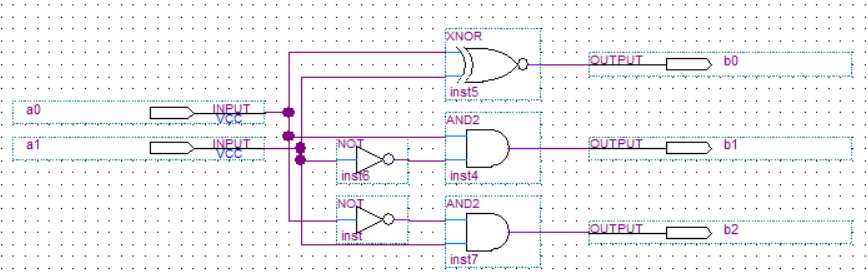
\includegraphics[width = 0.8 \textwidth]{graphics/base3.png}
		\caption{شماتیک ماژول \lr{base3}}
	\end{figure}
	\subsubsection{ماژول \lr{div3}}
	در این ماژول جمع دو عدد در مبنای ۳ محاسبه می‌شودم.
	\begin{equation*}
		\begin{cases}
			c_0 &= a_0b_0 + a_1 b_2 + a_2 b_1\\
			c_1 &= a_0b_1 + a_1b_0 + a_2b_2\\
			c_2 &= a_0b_2 + a_1b_1 + a_2 b_0
		\end{cases}
	\end{equation*}
		\begin{figure}[H]
		\centering
		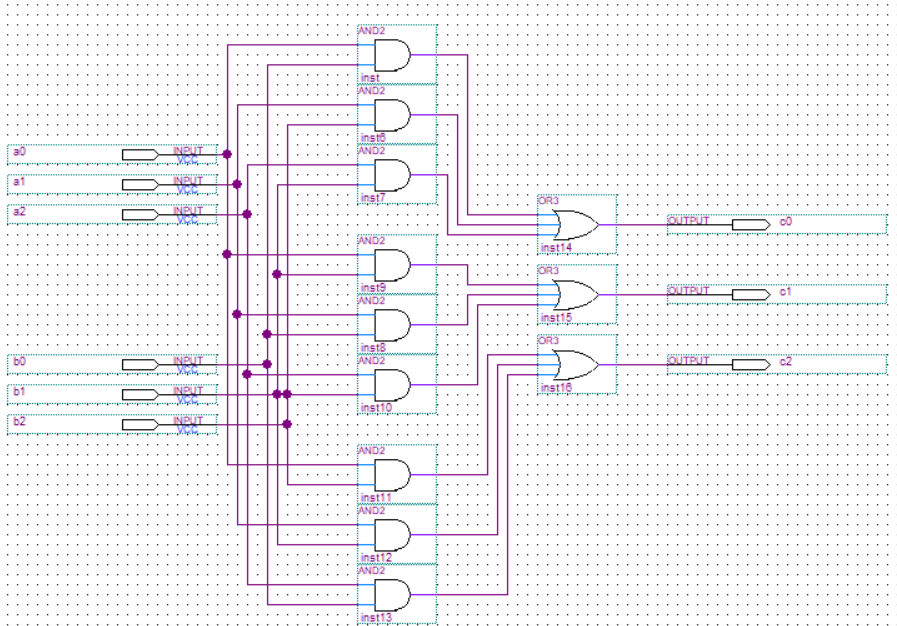
\includegraphics[width = 0.8 \textwidth]{graphics/div3.png}
		\caption{شماتیک ماژول \lr{div3}}
	\end{figure}
	\subsubsection{ماژول اصلی}
	ابتدا برای هر دو بیت ورودی با ماژول 
	\lr{base3}
	نمایش مبنای ۳ آن را بدست می‌آوریم. سپس با استفاده از ماژول 
	\lr{div3}
	این اعداد را با هم جمع می‌کنیم.
	\begin{figure}[H]
		\centering
		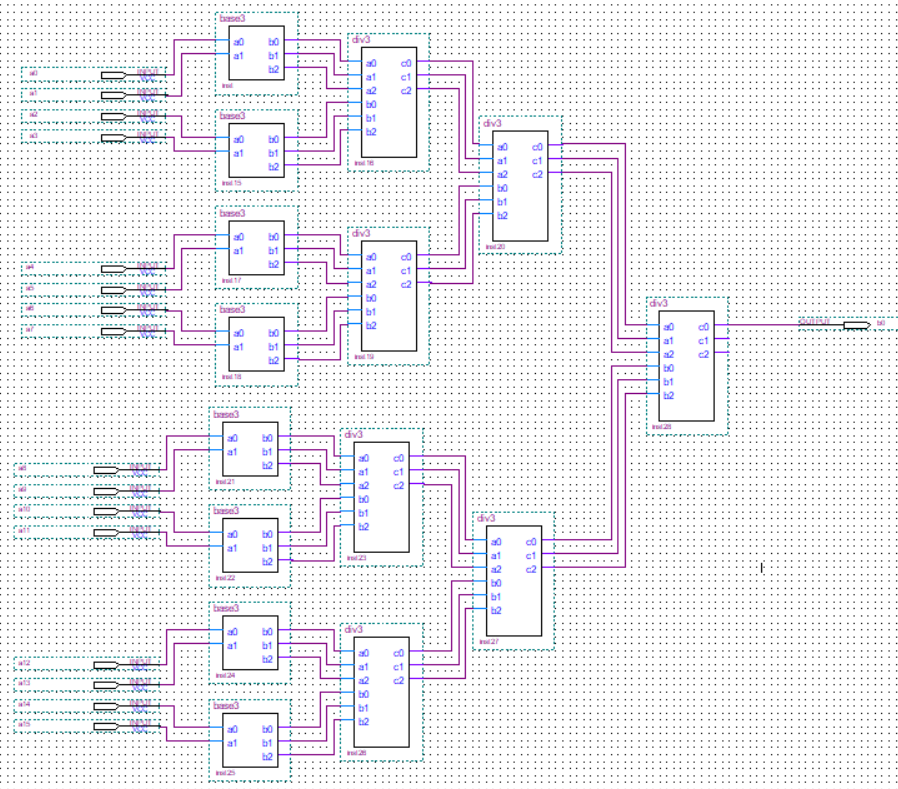
\includegraphics[width = 0.8 \textwidth]{graphics/lab3.png}
		\caption{شماتیک ماژول اصلی بخش‌پذیری بر ۳}
	\end{figure}
	\subsubsection{آزمون مدار}
	برای ورودی 
	\(4186,4185,4184,4036\)
	خروجی 
	\(0,1,0,0\)
	را بدست آوردیم.
	\begin{figure}[H]
		\centering
		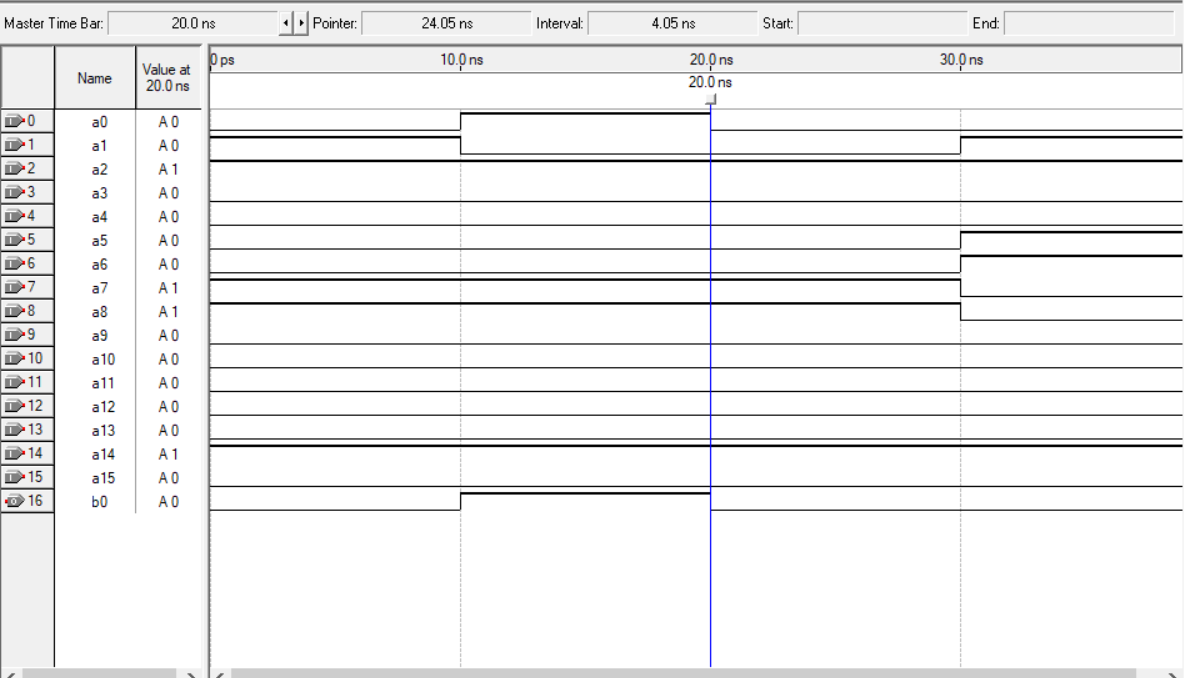
\includegraphics[width = 0.8 \textwidth]{graphics/waveform.png}
		\caption{Waveform آزمون مدار}
	\end{figure}
	\subsection{بخش‌پذیری بر ۱۱}
	ماژول‌ها زیر را طراحی کردیم.
	\subsubsection{ماژول \lr{fa}}
	مدار یک جمع‌کننده کامل تک بیتی است.
		\begin{figure}[H]
		\centering
		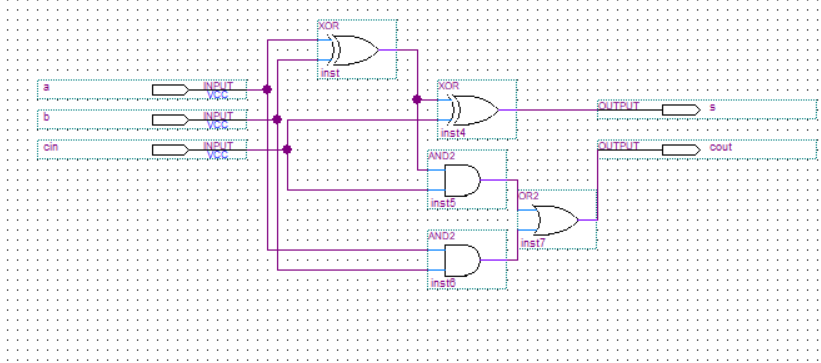
\includegraphics[width = 0.8 \textwidth]{graphics/fa.png}
		\caption{شماتیک مدار \lr{fa}}
	\end{figure}
	\subsubsection{ماژول \lr{sum4}}
	مدار یک جمع‌کننده کامل ۴ بیتی است.
			\begin{figure}[H]
		\centering
		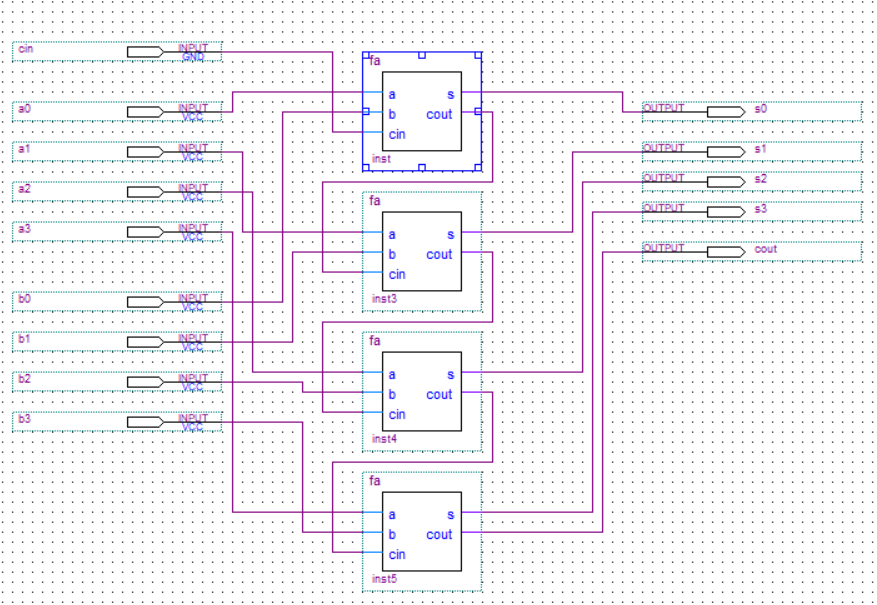
\includegraphics[width = 0.8 \textwidth]{graphics/sum4.png}
		\caption{شماتیک مدار \lr{sum4}}
	\end{figure}
	\subsection{ماژول \lr{mux1}}
	مدار یک مولتی‌پلکسر تک بیتی است.
			\begin{figure}[H]
		\centering
		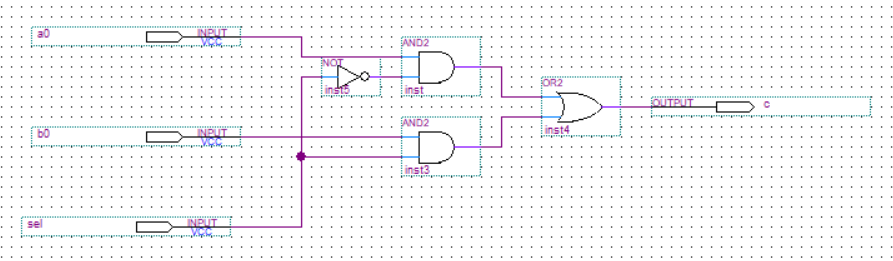
\includegraphics[width = 0.8 \textwidth]{graphics/mux1.png}
		\caption{شماتیک مدار \lr{mux1}}
	\end{figure}
		\subsection{ماژول \lr{mux4}}
	مدار یک مولتی‌پلکسر چهار بیتی است.
	\begin{figure}[H]
		\centering
		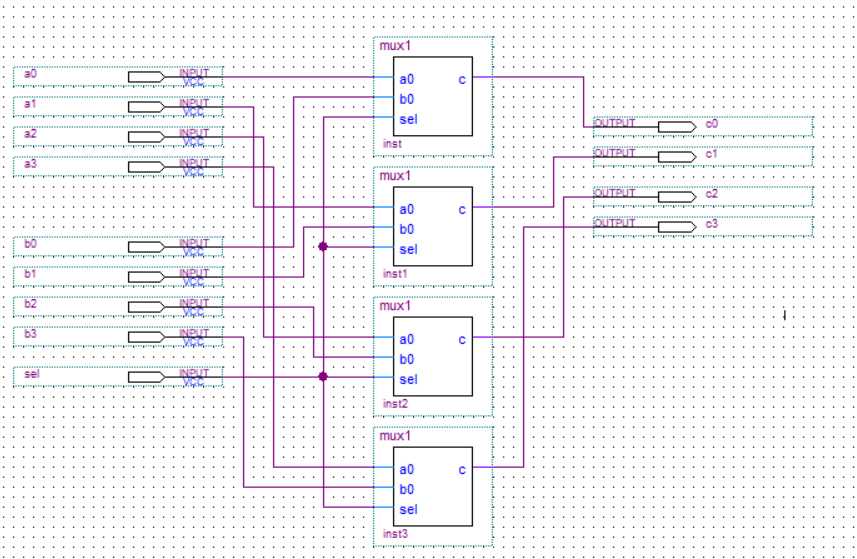
\includegraphics[width = 0.8 \textwidth]{graphics/mux4.png}
		\caption{شماتیک مدار \lr{mux4}}
	\end{figure}
	\subsection{ماژول \lr{diff11}}
	در این ماژول دو عدد باینری 
	\(0\leq a,b \leq 10\)
	به عنوان ورودی دریافت می‌کنیم. سپس 
	\(a - b\)
	را حساب می‌کنیم. در صورت که جواب منفی باشد، آن را با 
	11
	جمع می‌زنیم و خروجی می‌دهیم. در غیر این صورت، همان پاسخ تفریق را خروجی می‌دهیم.
	 	\begin{figure}[H]
	 	\centering
	 	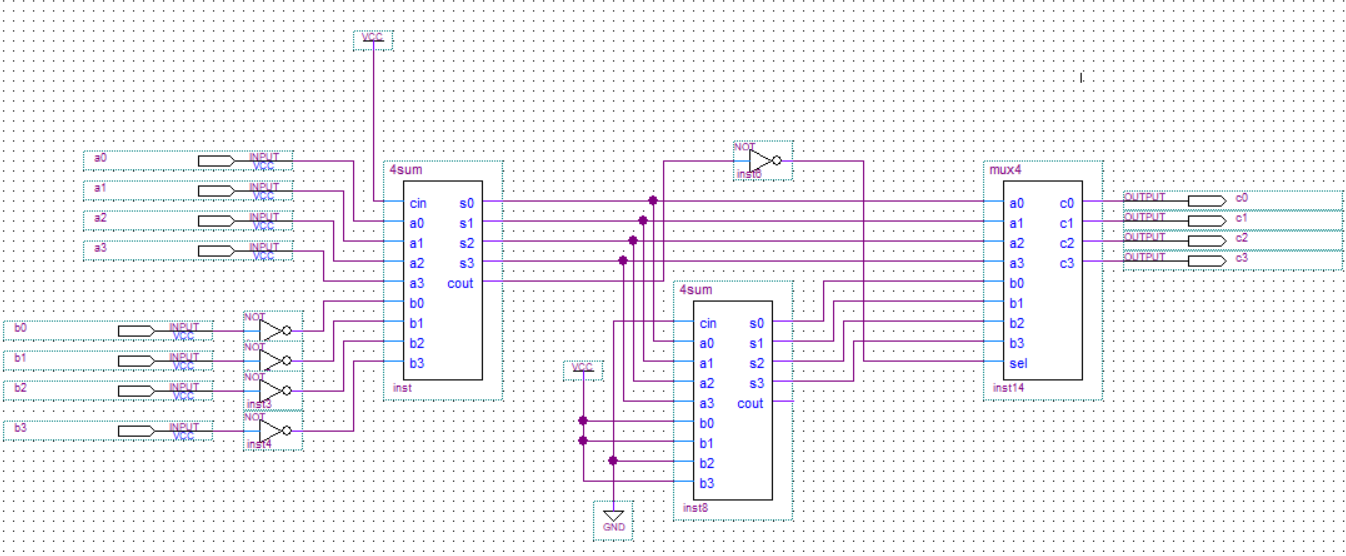
\includegraphics[width = 0.8 \textwidth]{graphics/diff11.png}
	 	\caption{شماتیک مدار \lr{diff11}}
	 \end{figure}
	 	\subsection{ماژول \lr{sum11}}
	 در این ماژول دو عدد باینری 
	 \(0\leq a,b \leq 10\)
	 به عنوان ورودی دریافت می‌کنیم. سپس 
	 \(a + b\)
	 را حساب می‌کنیم. در صورت که جواب بیشتر از ۱۱ باشد، از آن
	 11
	 را کم می‌کنیم و خروجی می‌دهیم. در غیر این صورت، همان پاسخ جمع را خروجی می‌دهیم.
	 \begin{figure}[H]
	 	\centering
	 	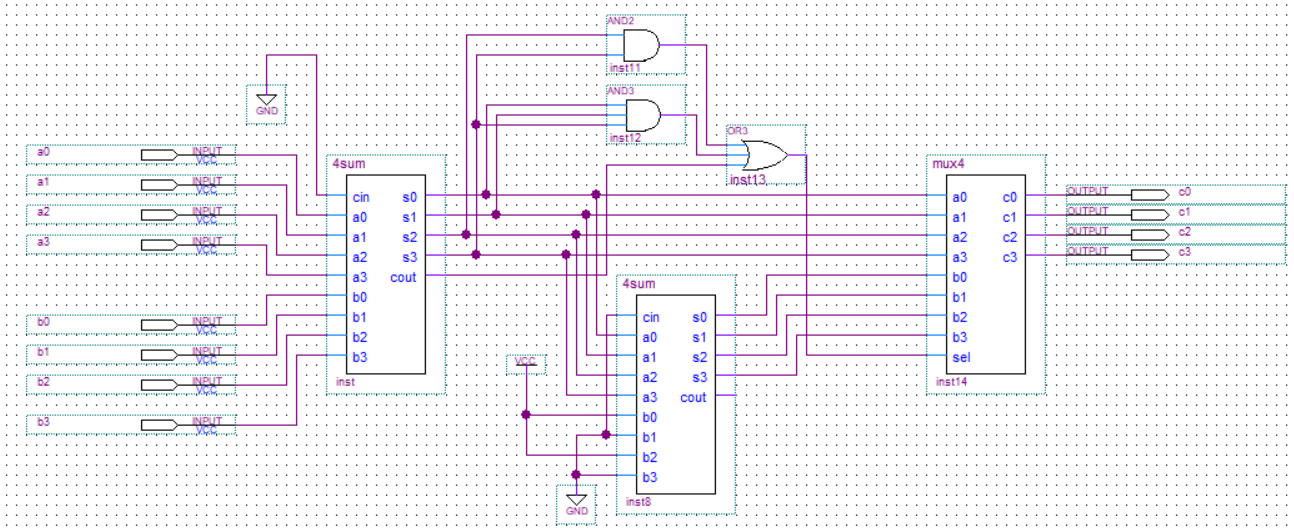
\includegraphics[width = 0.8 \textwidth]{graphics/sum11.png}
	 	\caption{شماتیک مدار \lr{sum11}}
	 \end{figure}
	 	 	\subsection{ماژول اصلی}
	 برای این مدار رقم‌ دوم را از رقم اول و رقم چهارم را از رقم سوم کم کردیم. سپس باقی‌مانده آن را بر ۱۱ حساب کردیم. این دو باقی‌مانده را با هم جمع کردیم و باقی‌مانده بر ۱۱ را حساب کردیم. در نهایت، بررسی می‌کنیم که باقی‌مانده صفر باشد.
	 \begin{figure}[H]
	 	\centering
	 	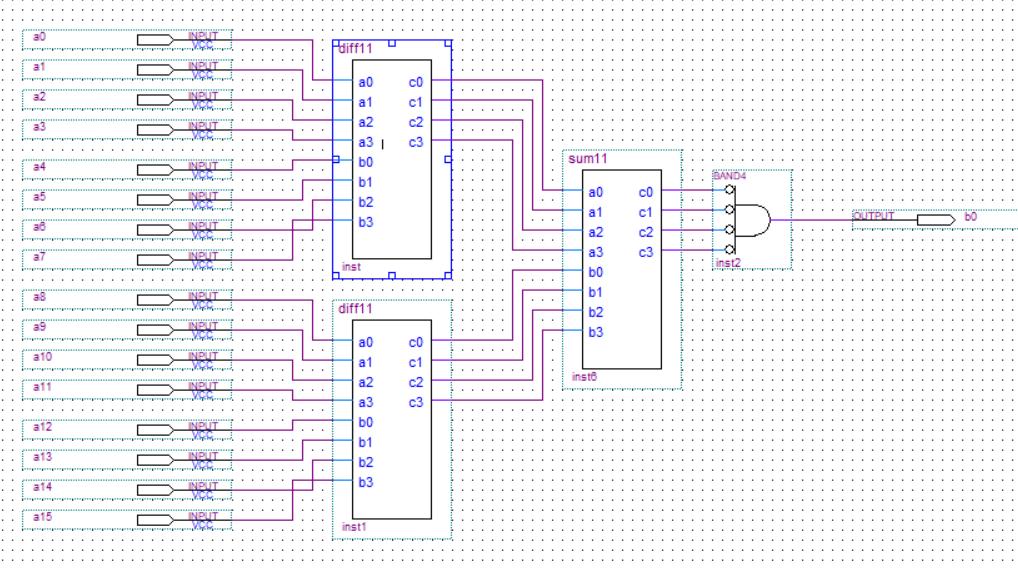
\includegraphics[width = 0.8 \textwidth]{graphics/lab11.png}
	 	\caption{شماتیک مدار ماژول اصلی بخش‌پذیری بر ۱۱}
	 \end{figure}
	 \subsubsection{آزمون مدار}
	 برای ورودی 
	 \(5423,1438,3098,6233\)
	 خروجی 
	 \(1,0,0,0\)
	 را بدست آوردیم.
	 \begin{figure}[H]
	 	\centering
	 	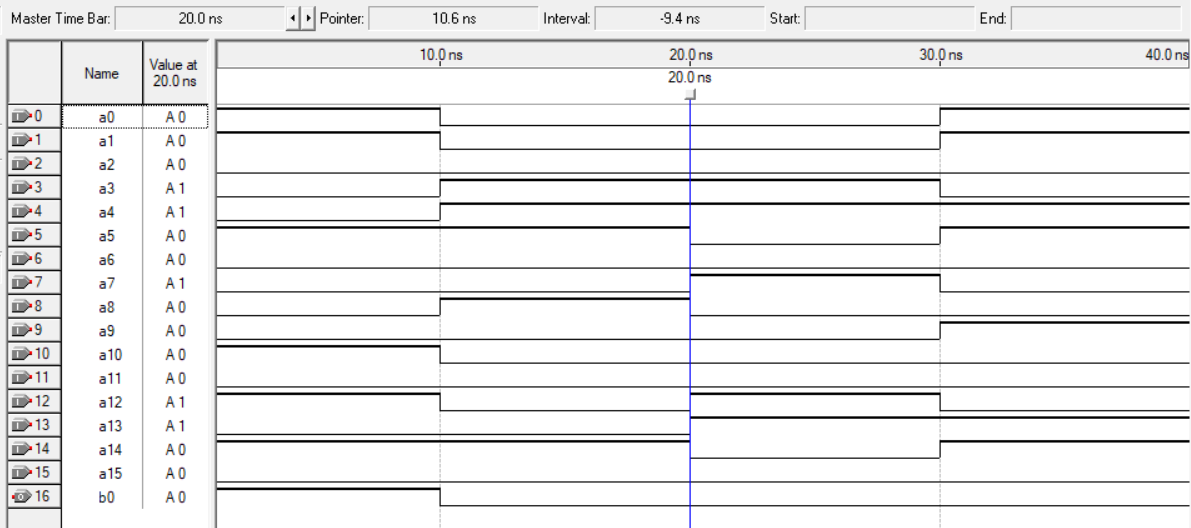
\includegraphics[width = 0.8 \textwidth]{graphics/waveform11.png}
	 	\caption{Waveform آزمون مدار}
	 \end{figure}
\end{document}